\documentclass[class=article, crop=false]{standalone}
\usepackage{my_preamble}
\begin{document}
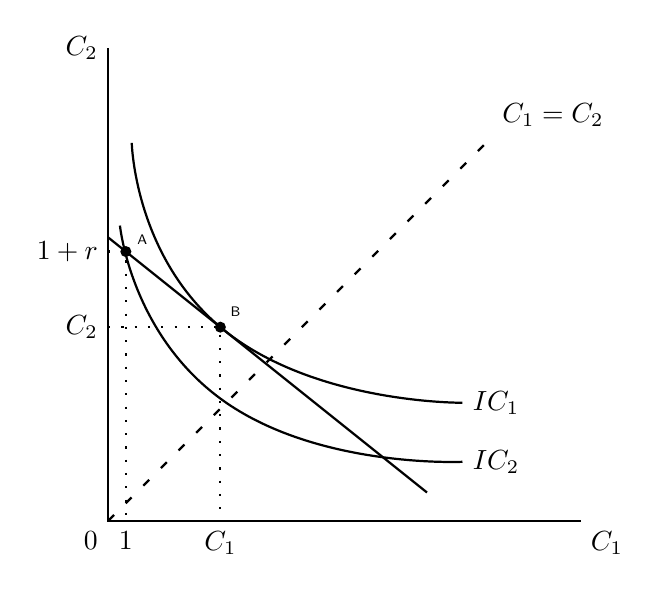
\begin{tikzpicture}[thick,font=\sffamily,scale=1.5]
	%axis
	 \draw (0,4) node[left]{$C_2$} -- (0,0) node[below left] {$0$} -- (4,0) node[below right]{$C_1$};
	  
	 %graphs
	\draw plot[domain=0:2.7,smooth] (\x,2.4-0.8*\x); %BC1
	\draw [loosely dashed] plot[domain=0:3.25,smooth] (\x,\x); %y=x line
	\draw plot [smooth, tension=1] coordinates{(0.2,3.2) (1,1.6) (3,1)}; %IC1	
	\draw plot [smooth, tension=1] coordinates{(0.1,2.5) (1,1) (3,0.5)}; %IC2
	
	%labels
	\node[right] at (3,1) {$IC_1$}; %BC label
	\node[right] at (3,0.5) {$IC_2$}; %IC label
	\node[above right] at (3.25,3.25) {$C_1=C_2$}; %IC label
	
	%dotted lines	
	 \draw[loosely dotted] (0,2.28) node[left]{$1+r$} -| node[pos=0.25,below=3mm] {}
	  (0.15,0) node[below]{$1$}; %dotted lines	
	

	%labels
	\node[style={fill=black,circle,inner sep=0pt,minimum size=4pt}] at (0.15,2.28) { };equib
	\node[above right]at (0.16,2.25) {\tiny{A}};
	\node[style={fill=black,circle,inner sep=0pt,minimum size=4pt}] at (0.95,1.64) { };equib
	\node[above right]at (0.95,1.64) {\tiny{B}};
	
	%dotted lines and arrows
	\draw[loosely dotted] (0,1.64) node[left]{$C_2$} -| node[pos=0.25,below=3mm] {}
	  (0.95,0) node[below]{$C_1$}; %dotted lines

\end{tikzpicture}
\end{document}